\chapter{Introduction}
\section{Initial Situation}
Common word processors do not prepare print-like documents in so far as these programs do not reflect the rules of professional printing which have been grown over centuries. These rules contain clear requirements for balancing page layouts, the amount of white space on pages, font-handling, etc. Donald Knuth's TeX package (see~citation removed to get rid of BibTeX warning) is a word processor which conforms to these printing rules. This package was enhanced by Leslie Lamport by providing more text structuring commands. He called his package LaTeX~citation removed to get rid of BibTeX warning.

When preparing a thesis, we want not only to have our content on a top level, we also want to commit to a high level of formal criteria. Therefore, we request our students to use one of these professional printing production environments like TeX or LaTeX.

Furthermore students should train their scientific writing skills. This includes a clear and structured break-down of their ideas, a high-level and clear wording, and the training of transparent citations of ideas from other sources than from theirs. A good source for more information concerning technical and scientific writing can be found in~citation removed to get rid of BibTeX warning.

\section{Goals}
The general goals and objectives of the project are described here. Care must be taken that the goals documented here are purely project goals and have nothing to do with individual goals of the team members. If individual goals should be part of the thesis they are listed in appendix~\ref{cha:individual-goals}.

\section{Overview}
Details of the diploma thesis have to be aligned between student and supervisor. This should be a basic structure to facilitate the first steps when students start to write their theses.

Never forget to add some illustrative images. Images must not be messed up with your normal text. They are encapsulated in floating bodies and referenced in your text. An example can be seen in figure~\ref{fig:sample}. As you can see, figures are placed by default on top of the page nearby the place where they are referenced the first time. Furthermore you can see that a list of figures is maintained automatically which can be included easily by typing the command \verb1\listoffigures1 into your document.

\begin{figure}
\begin{center}
	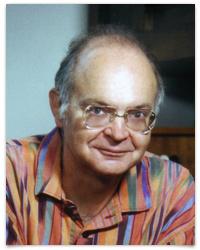
\includegraphics[scale=.5]{images/don_knuth.jpg}
\end{center}
	\caption{Don Knuth, the inventor of \TeX}
	\label{fig:sample}
\end{figure}

\section{Basic Terminology}
As usual the very basic terminology is briefly explained here. Most probably the explanations here only scratch a surface level. More detailed explanations of terminology goes into chapter~\ref{cha:theoretical-background}.

\section{Related Work and Projects}
Here a survey of other work in and around the area of the thesis is given. The reader shall see that the authors of the thesis know their field well and understand the developments there. Furthermore here is a good place to show what relevance the thesis in its field has.

\section{Structure of the Thesis}
Finally the reader is given a brief description what (s)he can expect in the thesis. Each chapter is introduced with a paragraph roughly describing its content.